\documentclass{standalone}
\usepackage{tikz}
\usetikzlibrary{patterns, positioning}


\begin{document}
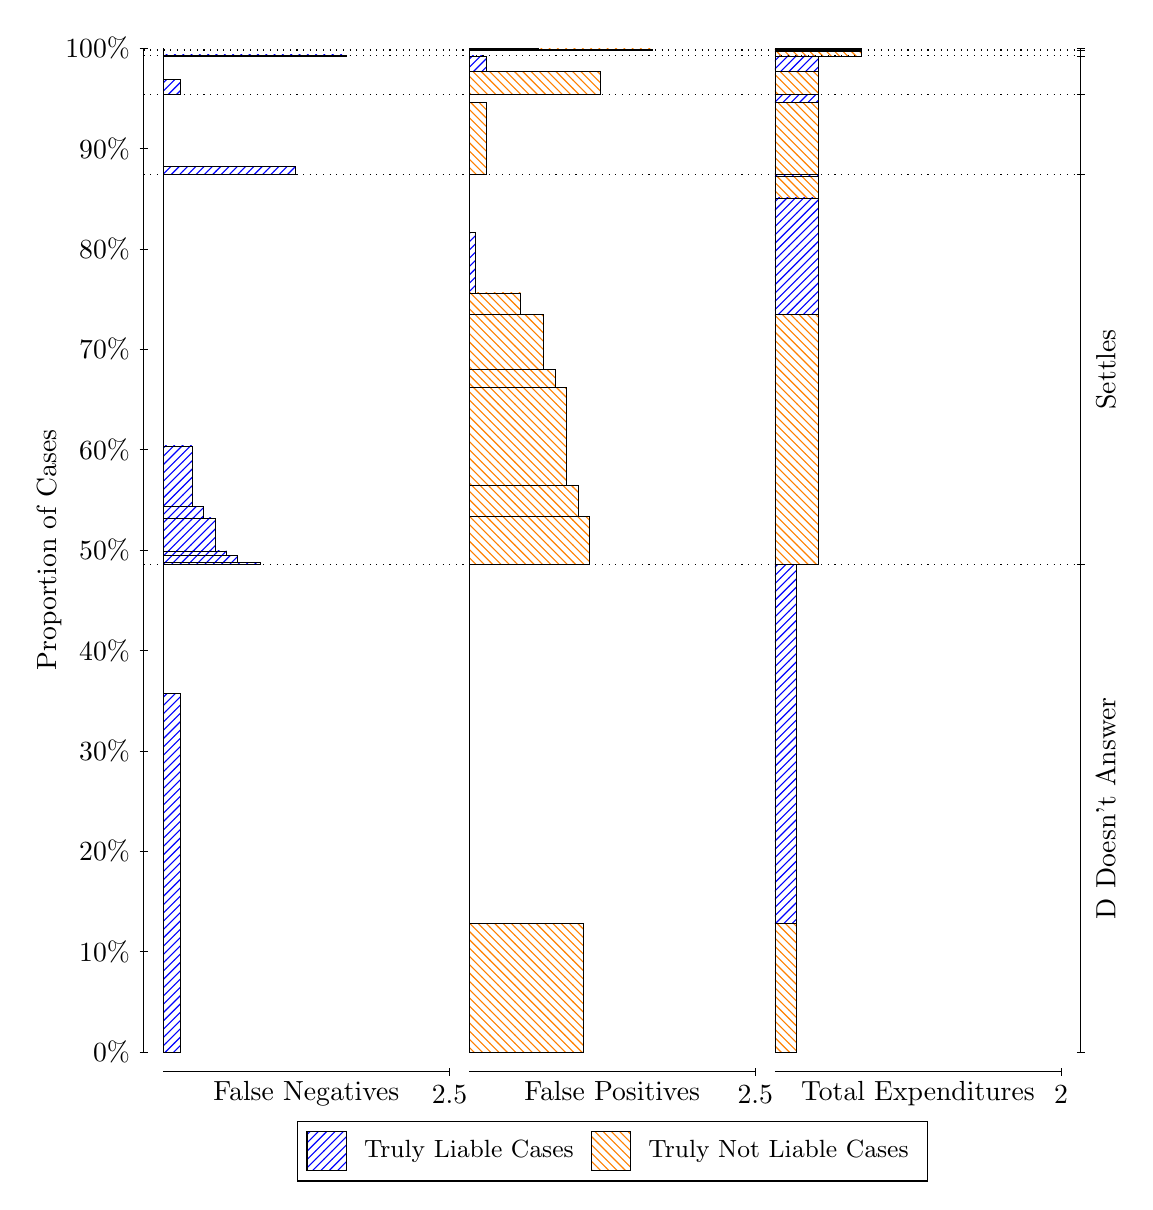
\begin{tikzpicture}
\draw[black, very thin] (1.5,1.75) -- (1.5,14.5);
\node[rotate=90, text=black, anchor=center] at (0.3, 8.125) {Proportion of Cases};
\draw[black, very thin] (1.45,1.75) -- (1.55,1.75);
\node[text=black, anchor=east] at (1.45, 1.75) {0\%};
\draw[black, very thin] (1.45,3.025) -- (1.55,3.025);
\node[text=black, anchor=east] at (1.45, 3.025) {10\%};
\draw[black, very thin] (1.45,4.3) -- (1.55,4.3);
\node[text=black, anchor=east] at (1.45, 4.3) {20\%};
\draw[black, very thin] (1.45,5.575) -- (1.55,5.575);
\node[text=black, anchor=east] at (1.45, 5.575) {30\%};
\draw[black, very thin] (1.45,6.85) -- (1.55,6.85);
\node[text=black, anchor=east] at (1.45, 6.85) {40\%};
\draw[black, very thin] (1.45,8.125) -- (1.55,8.125);
\node[text=black, anchor=east] at (1.45, 8.125) {50\%};
\draw[black, very thin] (1.45,9.4) -- (1.55,9.4);
\node[text=black, anchor=east] at (1.45, 9.4) {60\%};
\draw[black, very thin] (1.45,10.675) -- (1.55,10.675);
\node[text=black, anchor=east] at (1.45, 10.675) {70\%};
\draw[black, very thin] (1.45,11.95) -- (1.55,11.95);
\node[text=black, anchor=east] at (1.45, 11.95) {80\%};
\draw[black, very thin] (1.45,13.225) -- (1.55,13.225);
\node[text=black, anchor=east] at (1.45, 13.225) {90\%};
\draw[black, very thin] (1.45,14.5) -- (1.55,14.5);
\node[text=black, anchor=east] at (1.45, 14.5) {100\%};

\draw[black, very thin] (13.4,1.75) -- (13.4,14.5);
\draw[black, very thin] (13.35,1.75) -- (13.45,1.75);
\node[anchor=west] at (13.35, 1.75) {};
\draw[black, very thin] (13.35,7.94) -- (13.45,7.94);
\node[anchor=west] at (13.35, 7.94) {};
\draw[black, very thin] (13.35,12.899) -- (13.45,12.899);
\node[anchor=west] at (13.35, 12.899) {};
\draw[black, very thin] (13.35,13.907) -- (13.45,13.907);
\node[anchor=west] at (13.35, 13.907) {};
\draw[black, very thin] (13.35,14.401) -- (13.45,14.401);
\node[anchor=west] at (13.35, 14.401) {};
\draw[black, very thin] (13.35,14.475) -- (13.45,14.475);
\node[anchor=west] at (13.35, 14.475) {};
\draw[black, very thin] (13.35,14.5) -- (13.45,14.5);
\node[anchor=west] at (13.35, 14.5) {};

\draw[black, very thin, pattern color=blue, pattern=north east lines] (1.75,1.75) rectangle (1.968,6.3023);
\draw[black, very thin, pattern color=orange, pattern=north west lines] (1.75,6.3023) rectangle (1.75,7.94);
\draw[black, very thin, pattern color=blue, pattern=north east lines] (1.75,7.94) rectangle (2.9853,7.9663);
\draw[black, very thin, pattern color=blue, pattern=north east lines] (1.75,7.9663) rectangle (2.6947,8.061);
\draw[black, very thin, pattern color=blue, pattern=north east lines] (1.75,8.061) rectangle (2.5493,8.1124);
\draw[black, very thin, pattern color=blue, pattern=north east lines] (1.75,8.1124) rectangle (2.404,8.5328);
\draw[black, very thin, pattern color=blue, pattern=north east lines] (1.75,8.5328) rectangle (2.2587,8.6769);
\draw[black, very thin, pattern color=blue, pattern=north east lines] (1.75,8.6769) rectangle (2.1133,9.4477);
\draw[black, very thin, pattern color=orange, pattern=north west lines] (1.75,9.4477) rectangle (1.75,12.899);
\draw[black, very thin, pattern color=blue, pattern=north east lines] (1.75,12.899) rectangle (3.4213,12.996);
\draw[black, very thin, pattern color=orange, pattern=north west lines] (1.75,12.996) rectangle (1.75,13.907);
\draw[black, very thin, pattern color=blue, pattern=north east lines] (1.75,13.907) rectangle (1.968,14.1);
\draw[black, very thin, pattern color=orange, pattern=north west lines] (1.75,14.1) rectangle (1.75,14.401);
\draw[black, very thin, pattern color=blue, pattern=north east lines] (1.75,14.401) rectangle (4.0753,14.414);
\draw[black, very thin, pattern color=orange, pattern=north west lines] (1.75,14.414) rectangle (1.75,14.475);
\draw[black, very thin, pattern color=orange, pattern=north west lines] (1.75,14.475) rectangle (1.75,14.489);
\draw[black, very thin, pattern color=blue, pattern=north east lines] (1.75,14.489) rectangle (1.75,14.5);
\draw[black, very thin, pattern color=orange, pattern=north west lines] (5.6333,1.75) rectangle (7.0867,3.3876);
\draw[black, very thin, pattern color=blue, pattern=north east lines] (5.6333,3.3876) rectangle (5.6333,7.94);
\draw[black, very thin, pattern color=orange, pattern=north west lines] (5.6333,7.94) rectangle (7.1593,8.5477);
\draw[black, very thin, pattern color=orange, pattern=north west lines] (5.6333,8.5477) rectangle (7.014,8.9447);
\draw[black, very thin, pattern color=orange, pattern=north west lines] (5.6333,8.9447) rectangle (6.8687,10.188);
\draw[black, very thin, pattern color=orange, pattern=north west lines] (5.6333,10.188) rectangle (6.7233,10.42);
\draw[black, very thin, pattern color=orange, pattern=north west lines] (5.6333,10.42) rectangle (6.578,11.115);
\draw[black, very thin, pattern color=orange, pattern=north west lines] (5.6333,11.115) rectangle (6.2873,11.391);
\draw[black, very thin, pattern color=blue, pattern=north east lines] (5.6333,11.391) rectangle (5.706,12.162);
\draw[black, very thin, pattern color=blue, pattern=north east lines] (5.6333,12.162) rectangle (5.6333,12.899);
\draw[black, very thin, pattern color=orange, pattern=north west lines] (5.6333,12.899) rectangle (5.8513,13.81);
\draw[black, very thin, pattern color=blue, pattern=north east lines] (5.6333,13.81) rectangle (5.6333,13.907);
\draw[black, very thin, pattern color=orange, pattern=north west lines] (5.6333,13.907) rectangle (7.3047,14.208);
\draw[black, very thin, pattern color=blue, pattern=north east lines] (5.6333,14.208) rectangle (5.8513,14.401);
\draw[black, very thin, pattern color=orange, pattern=north west lines] (5.6333,14.401) rectangle (5.6333,14.461);
\draw[black, very thin, pattern color=blue, pattern=north east lines] (5.6333,14.461) rectangle (5.6333,14.475);
\draw[black, very thin, pattern color=orange, pattern=north west lines] (5.6333,14.475) rectangle (7.9587,14.489);
\draw[black, very thin, pattern color=blue, pattern=north east lines] (5.6333,14.489) rectangle (6.5053,14.5);
\draw[black, very thin, pattern color=orange, pattern=north west lines] (9.5167,1.75) rectangle (9.7892,3.3876);
\draw[black, very thin, pattern color=blue, pattern=north east lines] (9.5167,3.3876) rectangle (9.7892,7.94);
\draw[black, very thin, pattern color=orange, pattern=north west lines] (9.5167,7.94) rectangle (10.062,11.115);
\draw[black, very thin, pattern color=blue, pattern=north east lines] (9.5167,11.115) rectangle (10.062,12.596);
\draw[black, very thin, pattern color=orange, pattern=north west lines] (9.5167,12.596) rectangle (10.062,12.872);
\draw[black, very thin, pattern color=blue, pattern=north east lines] (9.5167,12.872) rectangle (10.062,12.899);
\draw[black, very thin, pattern color=orange, pattern=north west lines] (9.5167,12.899) rectangle (10.062,13.81);
\draw[black, very thin, pattern color=blue, pattern=north east lines] (9.5167,13.81) rectangle (10.062,13.907);
\draw[black, very thin, pattern color=orange, pattern=north west lines] (9.5167,13.907) rectangle (10.062,14.208);
\draw[black, very thin, pattern color=blue, pattern=north east lines] (9.5167,14.208) rectangle (10.062,14.401);
\draw[black, very thin, pattern color=orange, pattern=north west lines] (9.5167,14.401) rectangle (10.607,14.461);
\draw[black, very thin, pattern color=blue, pattern=north east lines] (9.5167,14.461) rectangle (10.607,14.475);
\draw[black, very thin, pattern color=orange, pattern=north west lines] (9.5167,14.475) rectangle (10.607,14.489);
\draw[black, very thin, pattern color=blue, pattern=north east lines] (9.5167,14.489) rectangle (10.607,14.5);
\draw[black, dotted] (1.5,7.94) -- (13.4,7.94);
\draw[black, dotted] (1.5,12.899) -- (13.4,12.899);
\draw[black, dotted] (1.5,13.907) -- (13.4,13.907);
\draw[black, dotted] (1.5,14.401) -- (13.4,14.401);
\draw[black, dotted] (1.5,14.475) -- (13.4,14.475);
\draw[black, very thin] (1.75,1.5) -- (5.3833,1.5);
\node[text=black, anchor=north] at (3.5667, 1.5) {False Negatives};
\draw[black, very thin] (5.3833,1.45) -- (5.3833,1.55);
\node[text=black, anchor=north] at (5.3833, 1.45) {2.5};

\draw[black, very thin] (5.6333,1.5) -- (9.2667,1.5);
\node[text=black, anchor=north] at (7.45, 1.5) {False Positives};
\draw[black, very thin] (9.2667,1.45) -- (9.2667,1.55);
\node[text=black, anchor=north] at (9.2667, 1.45) {2.5};

\draw[black, very thin] (9.5167,1.5) -- (13.15,1.5);
\node[text=black, anchor=north] at (11.333, 1.5) {Total Expenditures};
\draw[black, very thin] (13.15,1.45) -- (13.15,1.55);
\node[text=black, anchor=north] at (13.15, 1.45) {2};

\node[text=black, centered, rotate=90] at (13.72, 4.845) {D Doesn't Answer};
\node[text=black, centered, rotate=90] at (13.72, 10.419) {Settles};





\draw (7.449999999999999,1.5) node[draw=none] (baseCoordinate) {};
\begin{scope}[align=center]
        \matrix[scale=0.5, draw=black, below=0.5cm of baseCoordinate, nodes={draw}, column sep=0.1cm]{
            \node[rectangle, draw, minimum width=0.5cm, minimum height=0.5cm, pattern color=blue, pattern=north east lines] {}; &
            \node[draw=none, font=\small, text=black] (B) {Truly Liable Cases}; &
            \node[rectangle, draw, minimum width=0.5cm, minimum height=0.5cm, pattern color=orange, pattern=north west lines] {}; &
            \node[draw=none, font=\small, text=black] (B) {Truly Not Liable Cases}; \\
            };
\end{scope}

\end{tikzpicture}
\end{document}